
\section{数据预处理与分析}

为了后续模型的建立与求解,本文进行如下数据预处理,即数据清洗、数据量化等。具体机制如图\ref{fig:数据预处理机制}所示。

\begin{figure}[htbp]
	\centering
	% \includegraphics[width=0.8\textwidth]{图_数据预处理机制.png}
	\caption{数据预处理机制}
	\label{fig:数据预处理机制}
\end{figure}

\subsection{数据清洗}

本文首先进行了数据清洗。题中给出的附件包含三个表单,表单1包含文物编号、纹饰、类型、颜色和表面风化情况,表单2则包含了文物采样点和化学成分比例。通过观察发现,表单2的“文物采样点”列前缀的数字部分与表单1的文物编号相对应,因此我们通过正则表达式提取出其数字部分,创建出“文物编号”列,并基于此将表单1内容合并进来,形成包含完整信息的数据集。

随后我们对数据集中各变量进行缺失值统计,发现颜色和化学成分比例存在显著的缺失问题。题目中提到表单2中化学成分比例若存在空白处表示未检测到该成分,因此我们将这些缺失值填充为0,处理前后的化学成分频数如图\ref{fig:缺失值填充}所示。

\begin{figure}[htbp]
	\centering
	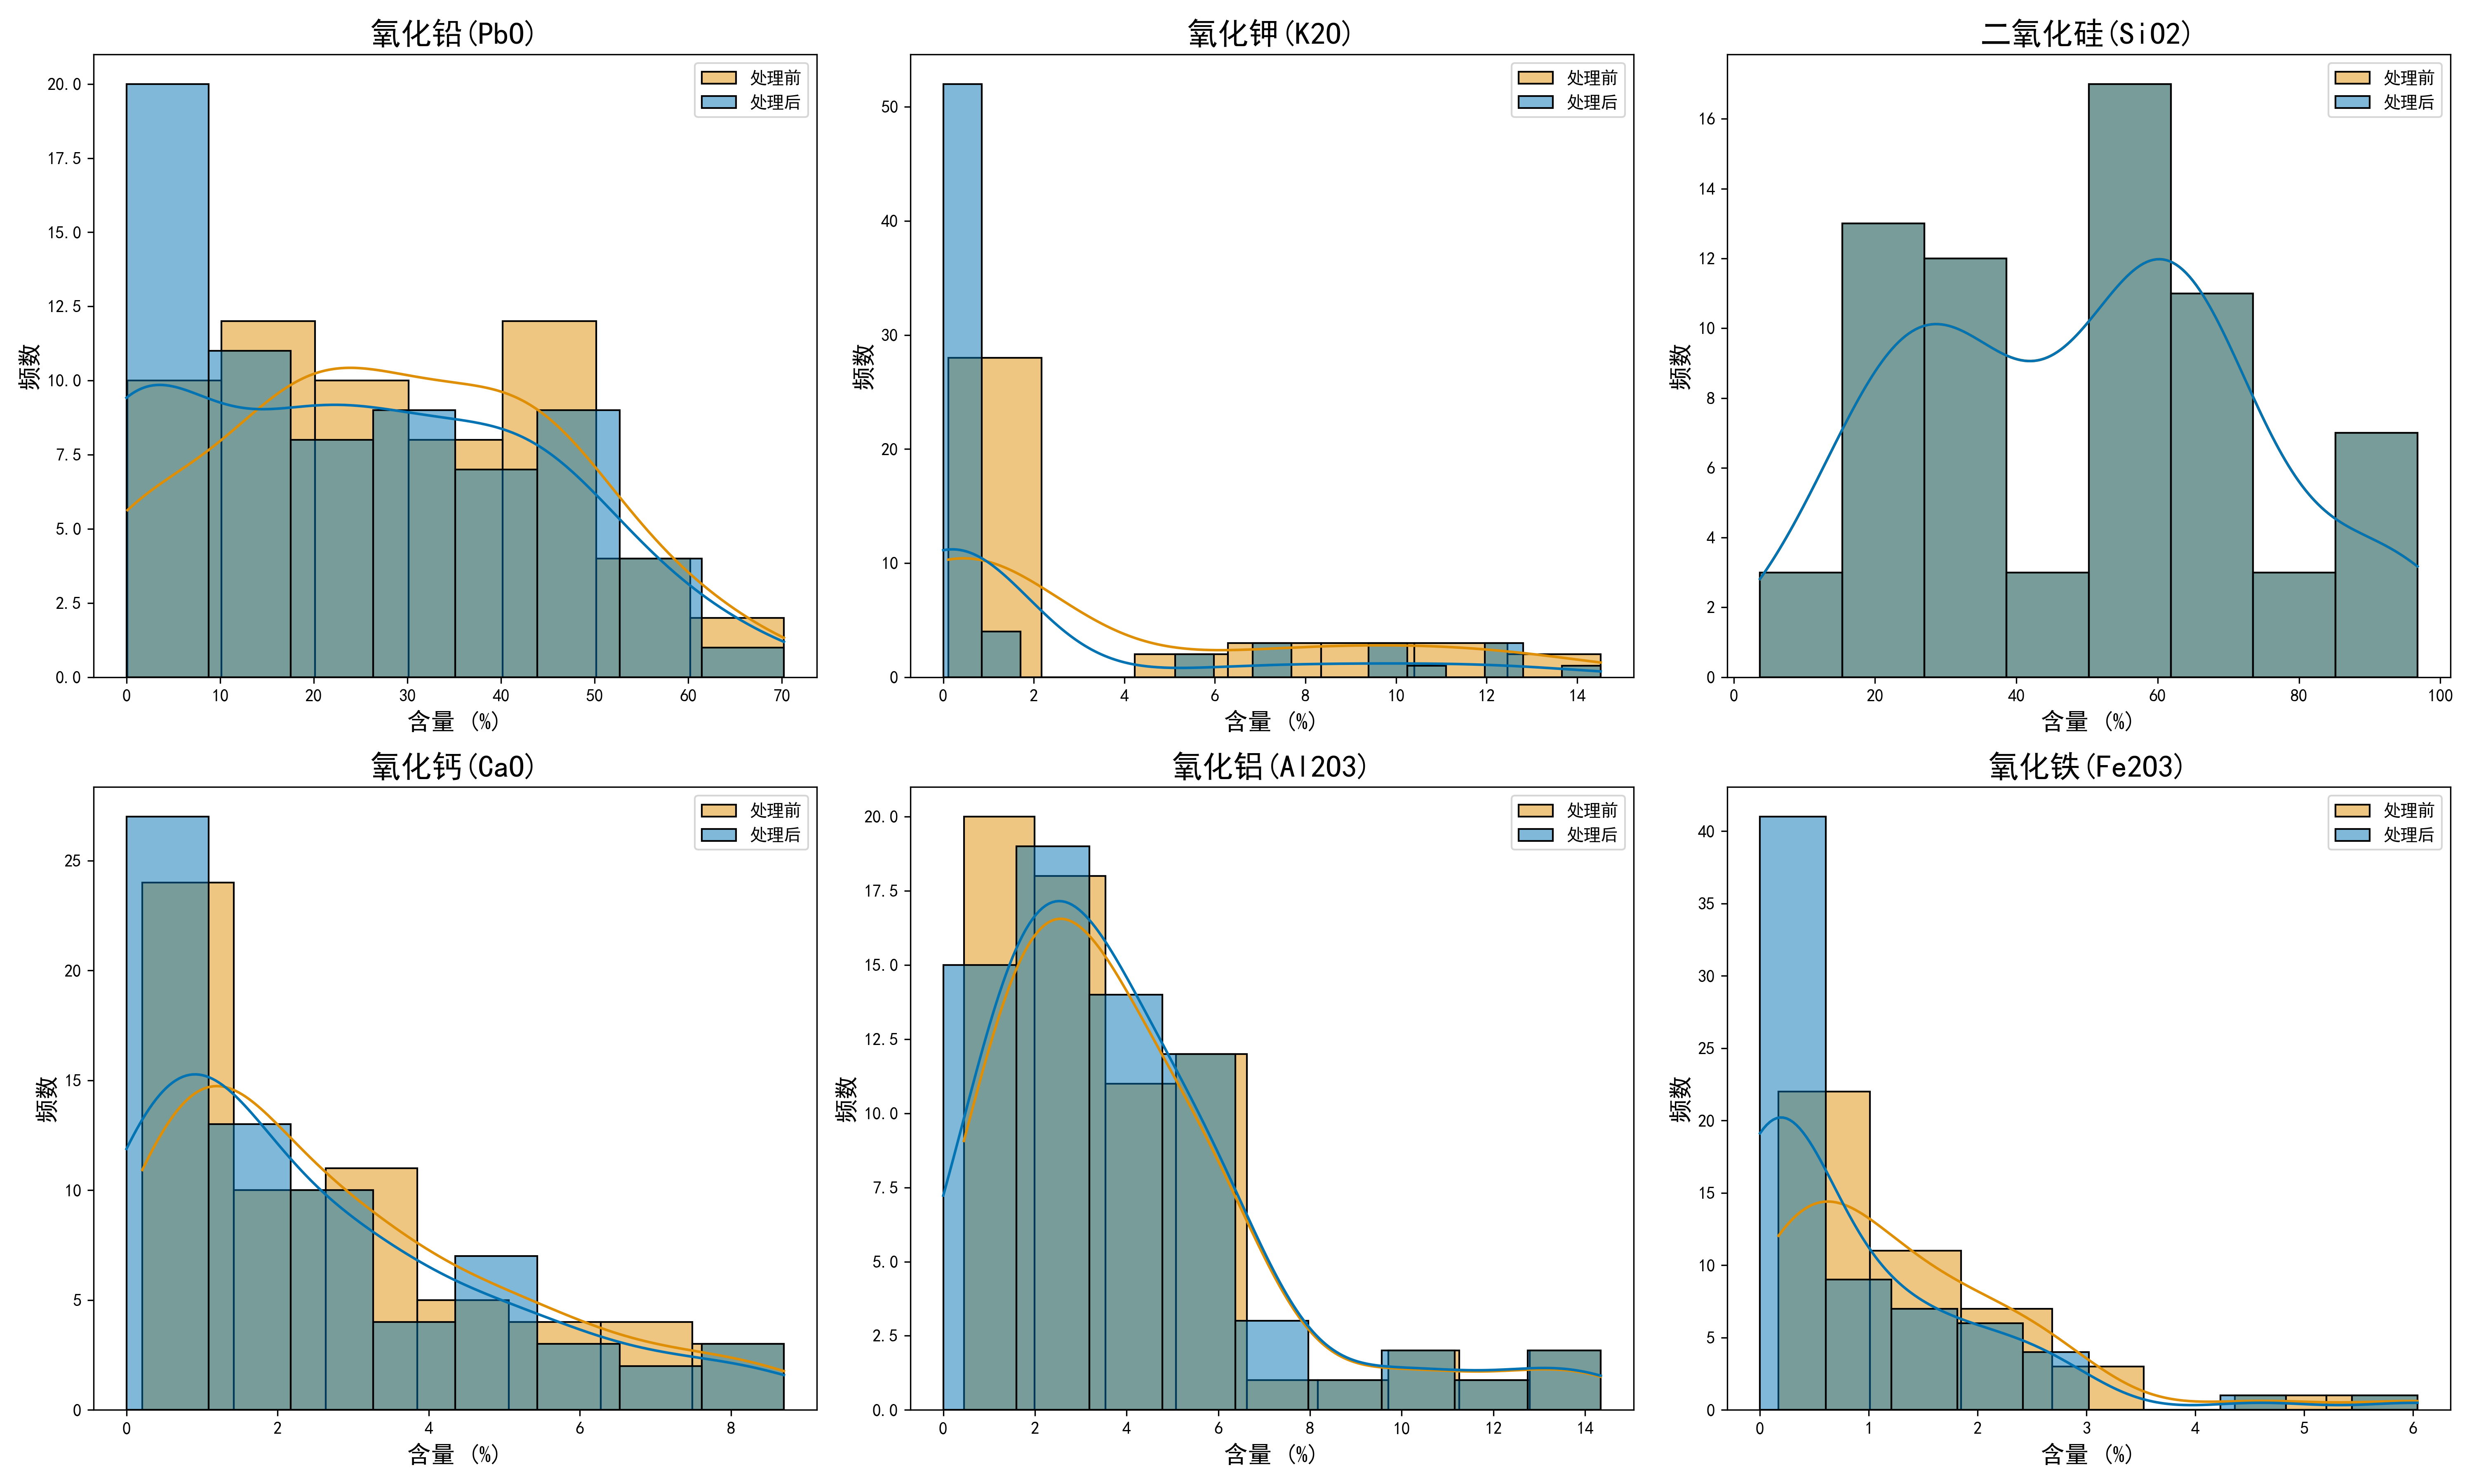
\includegraphics[width=0.8\textwidth]{figs/2模型准备/化学成分缺失值填充.png}
	\caption{化学成分缺失值填充}
	\label{fig:缺失值填充}
\end{figure}

而对于颜色缺失,我们首先想到通过全局众数填充,但是其误差可能较大,于是我们采用了一种条件众数填充法。具体而言,对于一个颜色信息缺失的样本,系统会自动寻找数据集中所有与该样本在类型、表面风化和纹饰上完全一致的其他样本,然后用这个小群体中出现次数最多的颜色来填充缺失值。其填充内容如图\ref{fig:颜色缺失值填充}所示。

\begin{table}[htbp]
	\centering
	\caption{按类型和纹饰划分的颜色众数及对应文物编号}
	\label{tab:颜色缺失值填充}
	\begin{tabular}{llll}
		\toprule
		\textbf{类型} & \textbf{纹饰} & \textbf{颜色众数} & \textbf{对应文物编号}                                        \\
		\midrule
		\rowcolor{gray!20}
		铅钡          & A           & 浅蓝            & \parbox[t]{6cm}{2, 19, 20, 23, 28, 29, 30, 42, 44, 45, \\ 46, 47, 48, 49, 50, 53} \\
		铅钡          & C           & 浅蓝            & \parbox[t]{6cm}{8, 11, 24, 25, 26, 31, 32, 33, 34, 35, \\ 36, 37, 38, 39, 40, 41, 43, 51, 52,  \\ 54,55, 56, 57, 58} \\
		\rowcolor{gray!20}
		高钾          & A           & 蓝绿            & 3, 4, 5, 6, 18, 21                                     \\
		高钾          & B           & 蓝绿            & 7, 9, 10, 12, 22, 27                                   \\
		\rowcolor{gray!20}
		高钾          & C           & 浅蓝            & 1, 13, 14, 15, 16, 17                                  \\
		\bottomrule
	\end{tabular}
\end{table}

针对各种化学成分比例,本题中将成分比例累加和介于85\%~105\%之间的数据视为有效数据,因此我们对其进行成分性异常值检测。我们计算每个样本所有化学成分的累加和,并筛选出总和介于85\%到105\%之间的数据作为有效样本,得到67条有效已分类样本、8条有效未分类样本以及2条异常样本,然后剔除异常样本。

最后我们检测了高钾玻璃和铅钡玻璃以及它们中风化和未风化的占比,如图\ref{fig:玻璃类型分布}所示:
\begin{figure}[htbp]
	\centering
	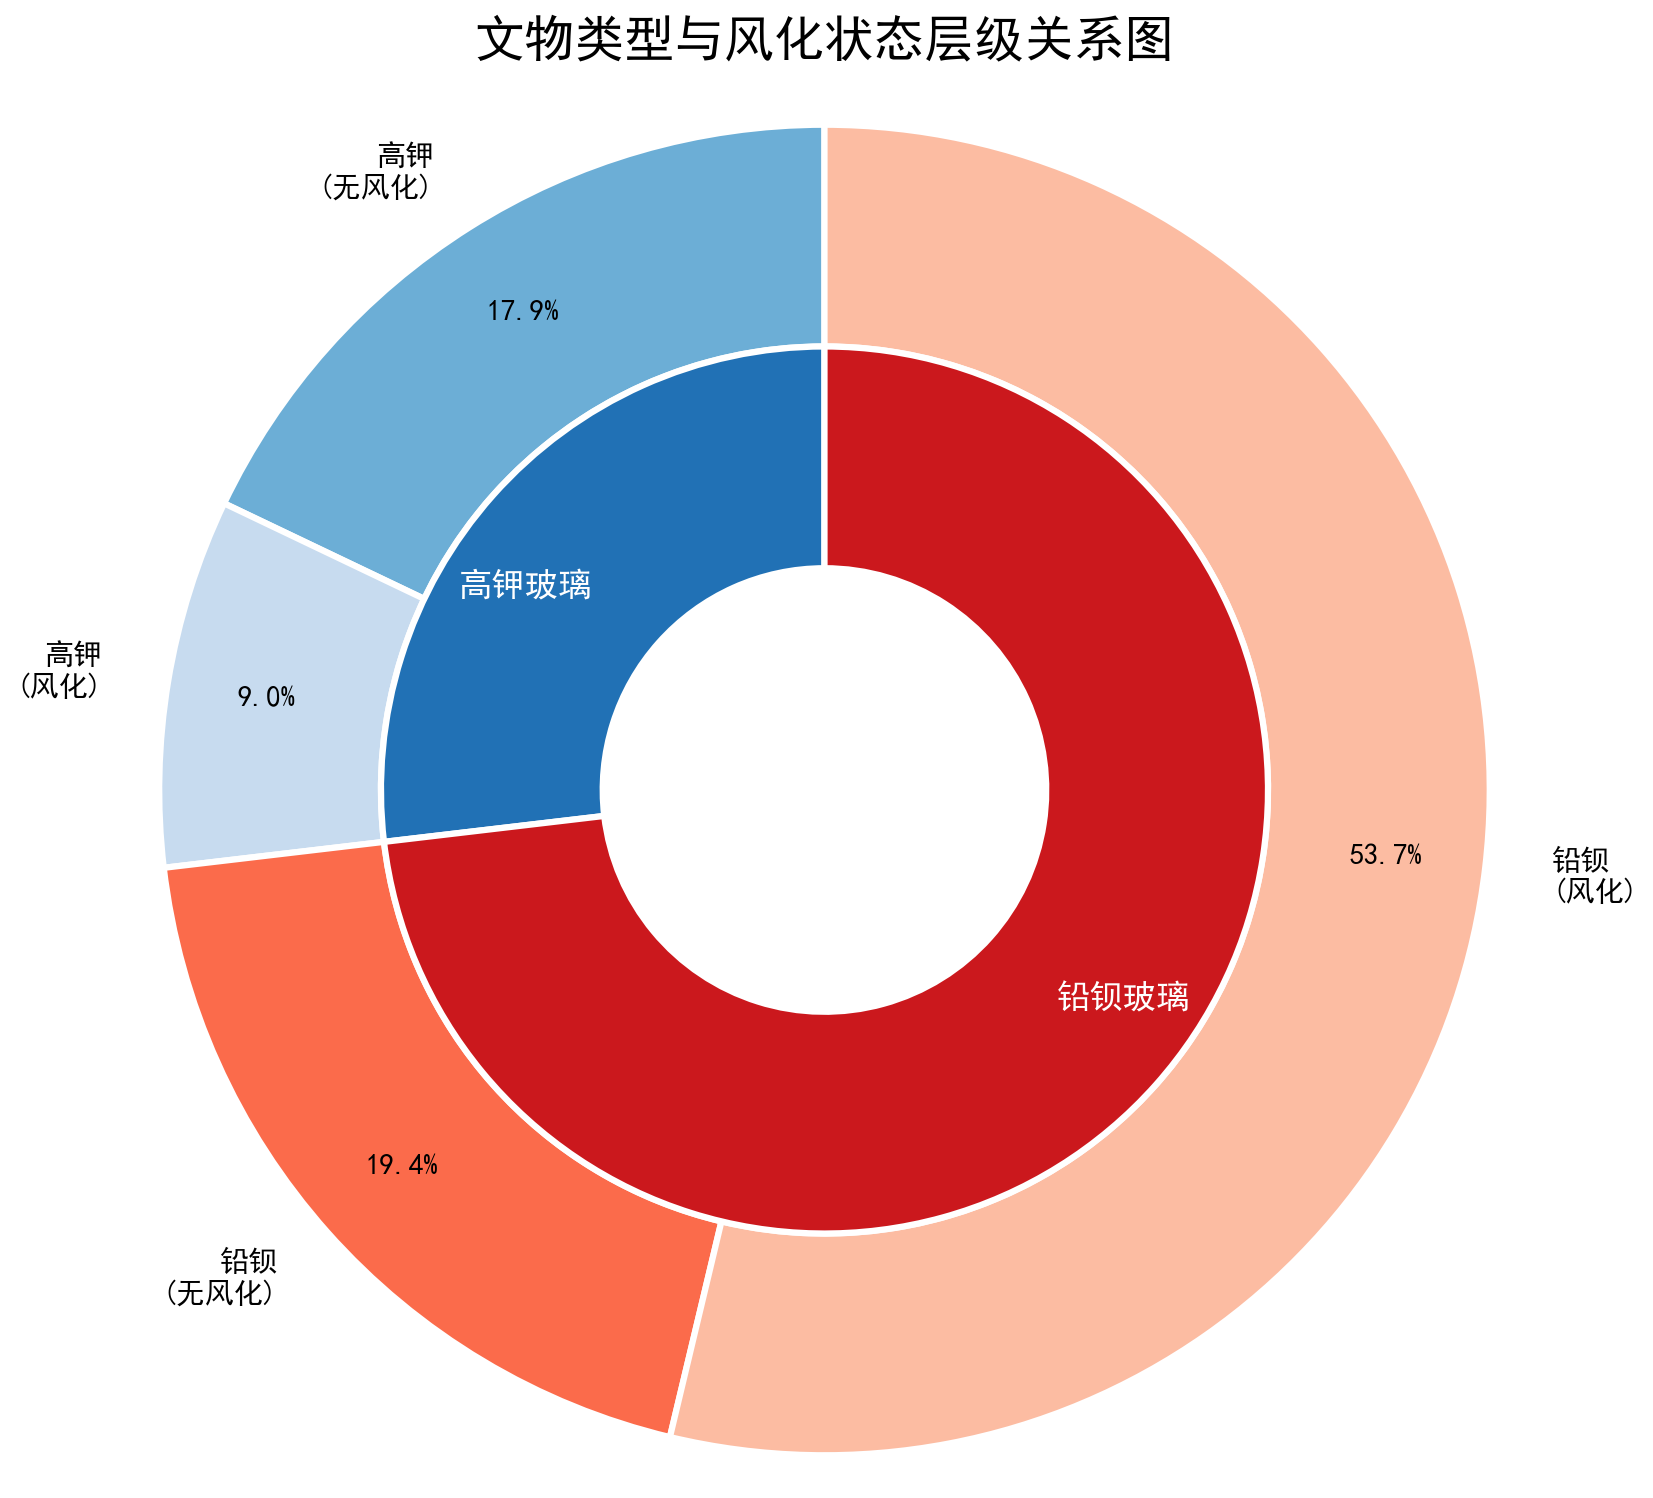
\includegraphics[width=0.8\textwidth]{figs/2模型准备/类型与风化嵌套饼图.png}
	\caption{玻璃类型分布}
	\label{fig:玻璃类型分布}
\end{figure}
从图中可以看出,类型、风化这两个核心分类变量的样本量均衡,故后续建模无需进行特殊的不平衡处理。

数据清洗的整体效果如图\ref{fig:数据清洗效果}所示。
\begin{figure}[htbp]
	\centering
	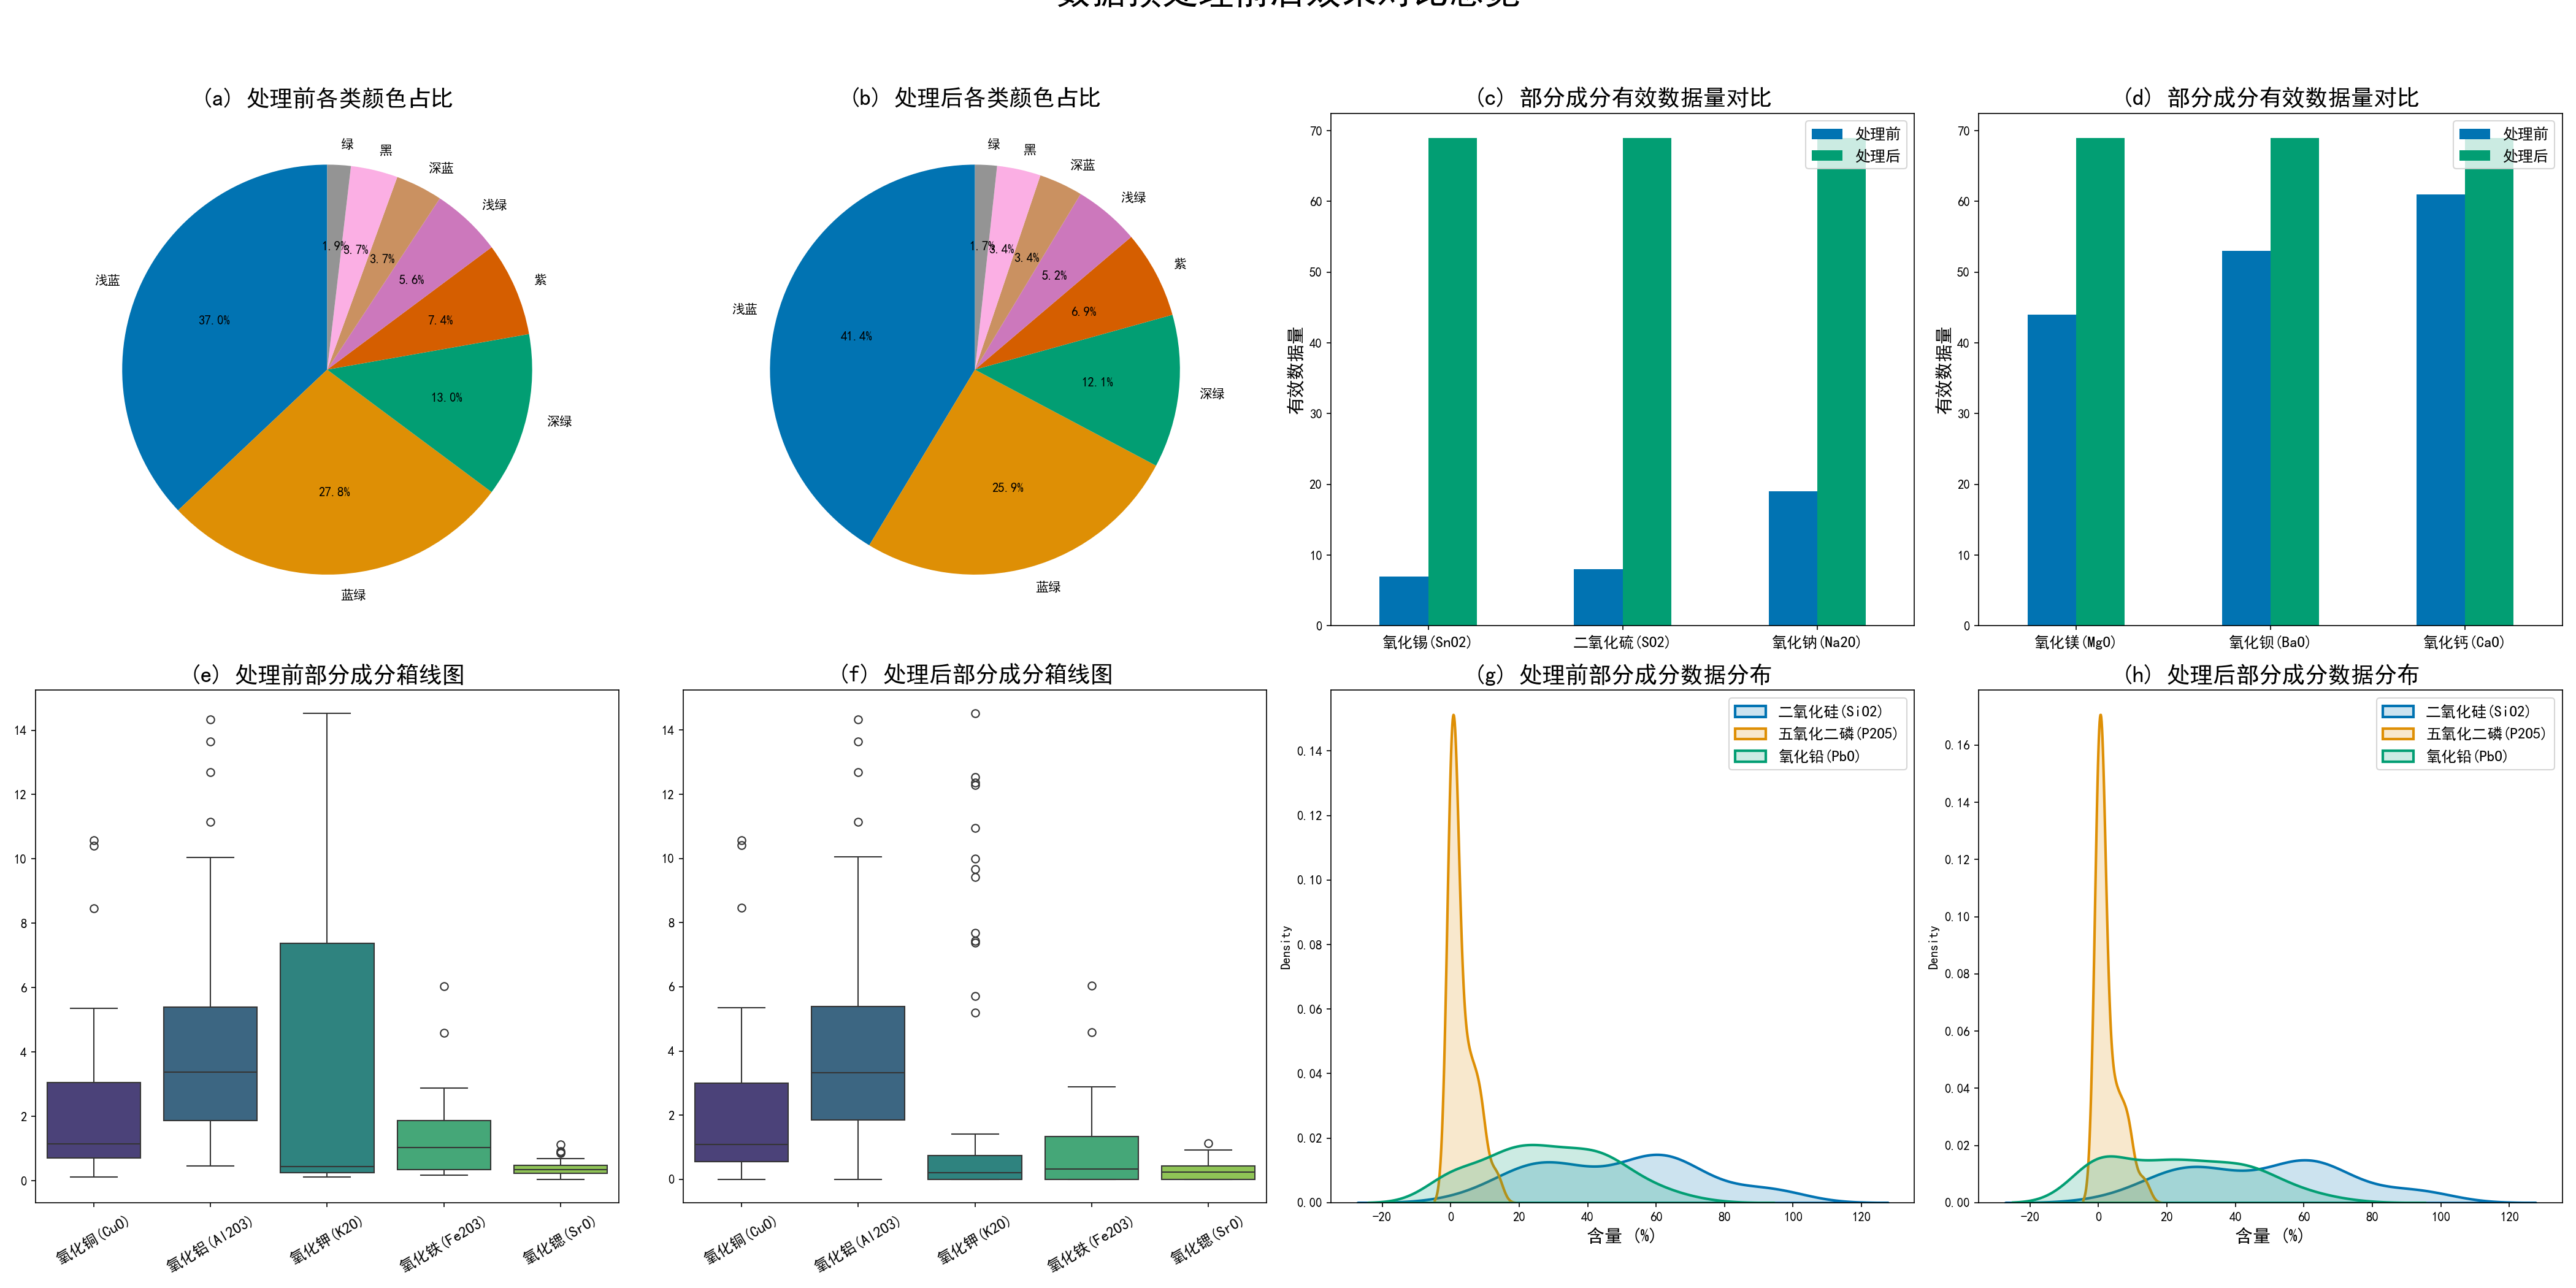
\includegraphics[width=\textwidth]{figs/2模型准备/预处理效果.png}
	\caption{数据清洗效果}
	\label{fig:数据清洗效果}
\end{figure}


\subsection{数据量化}

本文为了便于后续相关数学模型的建立与求解,增强可理解性,进一步将合并后的文件中的名称进行数据量化。对于作为因变量的“类型”列,我们使用标签编码,将“铅钡”映射为 0,“高钾”映射为 1。对于作为自变量的各项分类特征列,为了避免引入虚假的、不存在的顺序和距离关系,我们排除了顺序编码和RGB向量的方案,最终选择了最忠实于数据本身特性的独热编码。数据量化的具体细节如表所示:
\begin{table}[h!]
	\centering
	\caption{数据量化方法示例}
	\label{tab:quantification_example}
	\renewcommand{\arraystretch}{1.5} % 增加行高以获得更好的视觉效果
	\begin{tabular}{lccc}
		\toprule
		\textbf{列名} & \textbf{原始数据形态}               & \textbf{量化方法} & \textbf{量化后形态}                                \\
		\midrule
		\rowcolor{gray!20}
		类型          & \texttt{['高钾', '铅钡']}         & 标签编码          & \texttt{[1, 0]}                               \\
		表面风化        & \texttt{['风化', '无风化']}        & 独热编码          & 表面风化\_风化 \texttt{[1 / 0]} \\
		\rowcolor{gray!20}
		颜色          & \texttt{['蓝绿', '浅蓝', ...]}    & 独热编码          & \parbox{4cm}{\centering 颜色\_蓝绿 \texttt{[1/0]} \\ 颜色\_浅蓝 \texttt{[1/0]} \\ ···} \\
		纹饰          & \texttt{['A', 'B', 'C', ...]} & 独热编码          & \parbox{4cm}{\centering 纹饰\_A \texttt{[1/0]}  \\ 纹饰\_B \texttt{[1/0]} \\ ···} \\
		\rowcolor{gray!20}
		各类化学成分比例    & 如 69.33                       & 无需处理          & 69.33                                         \\
		\bottomrule
	\end{tabular}
\end{table}




